
\begin{figure}
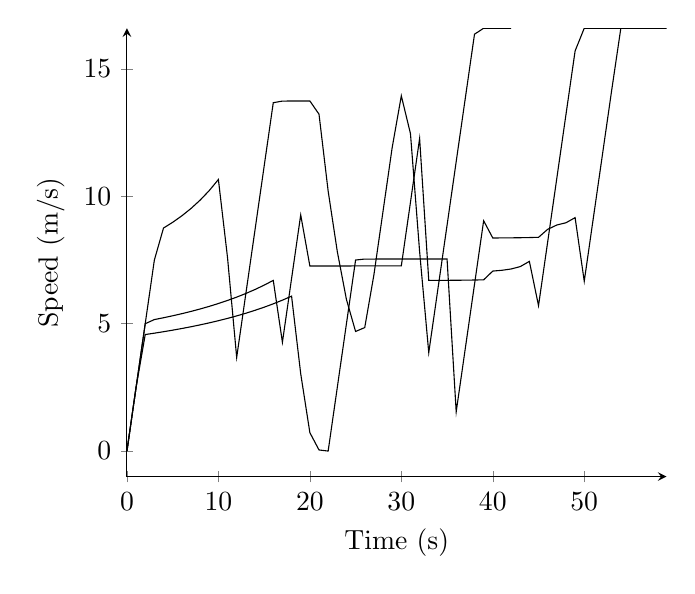
\begin{tikzpicture}
\begin{axis}[
legend style={anchor=west},
axis x line=bottom,
axis y line=left,
ymin=-1,
xlabel=Time (s),
ylabel=Speed (m/s),
]
\addplot[] coordinates {
(0, 0.0)
(1, 2.5)
(2, 4.57437532972)
(3, 4.62828412043)
(4, 4.68554097148)
(5, 4.7464314448)
(6, 4.81127243699)
(7, 4.88041642121)
(8, 4.95425637701)
(9, 5.03323153906)
(10, 5.11783412431)
(11, 5.20861723294)
(12, 5.30620416393)
(13, 5.41129944241)
(14, 5.52470192916)
(15, 5.64732047422)
(16, 5.78019269628)
(17, 5.92450762293)
(18, 6.08163312756)
(19, 3.03584896658)
(20, 0.724312526041)
(21, 0.043560923444)
(22, 0.0)
(23, 2.5)
(24, 5.0)
(25, 7.5)
(26, 7.53794000826)
(27, 7.53815931989)
(28, 7.53840632181)
(29, 7.5386858833)
(30, 7.53900399391)
(31, 7.53936808793)
(32, 7.53978748409)
(33, 7.54027398995)
(34, 7.54084274543)
(35, 7.54151342024)
(36, 1.54151342024)
(37, 4.04151342024)
(38, 6.54151342024)
(39, 9.04151342024)
(40, 8.36515282085)
(41, 8.3677571736)
(42, 8.37117743272)
(43, 8.37579548964)
(44, 8.38224744473)
(45, 8.39165930815)
(46, 8.70488406915)
(47, 8.8744627782)
(48, 8.96267462379)
(49, 9.16351723394)
(50, 6.66686771966)
(51, 9.16686771966)
(52, 11.6668677197)
(53, 14.1668677197)
(54, 16.6)
(55, 16.6)
(56, 16.6)
(57, 16.6)
(58, 16.6)
(59, 16.6)
};
\addplot[] coordinates {
(0, 0.0)
(1, 2.5)
(2, 5.0)
(3, 7.5)
(4, 8.7552810082)
(5, 8.98037148557)
(6, 9.23419422736)
(7, 9.52189838335)
(8, 9.84984867398)
(9, 10.2259885054)
(10, 10.6603366443)
(11, 7.59062076812)
(12, 3.67561489754)
(13, 6.17561489754)
(14, 8.67561489754)
(15, 11.1756148975)
(16, 13.6756148975)
(17, 13.7402869195)
(18, 13.7414471048)
(19, 13.7429509217)
(20, 13.7449490167)
(21, 13.2250069504)
(22, 10.2067022311)
(23, 7.83376288733)
(24, 5.9503656045)
(25, 4.69564145839)
(26, 4.84786577242)
(27, 6.91340732607)
(28, 9.41340732607)
(29, 11.9134073261)
(30, 13.9452350942)
(31, 12.4604279073)
(32, 7.82976007143)
(33, 3.86433691518)
(34, 6.36433691518)
(35, 8.86433691518)
(36, 11.3643369152)
(37, 13.8643369152)
(38, 16.3643369152)
(39, 16.6)
(40, 16.6)
(41, 16.6)
(42, 16.6)
};
\addplot[] coordinates {
(0, 0.0)
(1, 2.5)
(2, 5.0)
(3, 5.16222950026)
(4, 5.23399054673)
(5, 5.31086486447)
(6, 5.3933544299)
(7, 5.48202482783)
(8, 5.57751522883)
(9, 5.68055024834)
(10, 5.79195410499)
(11, 5.91266760338)
(12, 6.04376860516)
(13, 6.18649683373)
(14, 6.34228409531)
(15, 6.51279131364)
(16, 6.6999541949)
(17, 4.27008486967)
(18, 6.77008486967)
(19, 9.27008486967)
(20, 7.26644580871)
(21, 7.26664752625)
(22, 7.26687363194)
(23, 7.26712822474)
(24, 7.26741630314)
(25, 7.26774401309)
(26, 7.26811897952)
(27, 7.26855075553)
(28, 7.26905143917)
(29, 7.26963653382)
(30, 7.27032616853)
(31, 9.77032616853)
(32, 12.2703261685)
(33, 6.69875658614)
(34, 6.70063884433)
(35, 6.70299674534)
(36, 6.70600594044)
(37, 6.70993182663)
(38, 6.71519119457)
(39, 6.72247009207)
(40, 7.06640894874)
(41, 7.09736245167)
(42, 7.1482583597)
(43, 7.24162626128)
(44, 7.44704096236)
(45, 5.7084682476)
(46, 8.2084682476)
(47, 10.7084682476)
(48, 13.2084682476)
(49, 15.7084682476)
(50, 16.6)
(51, 16.6)
(52, 16.6)
(53, 16.6)
(54, 16.6)
};

\end{axis}
\end{tikzpicture}
\label{tik:100:55}
\caption{100 percent diving with GSC on route $55$}
\end{figure}
